% !TeX root = ../seminar.tex
\section{Summary}

\begin{frame}{Summary}
\begin{itemize}
  \item<+-> $\sim\!10^8$ stellar black holes in the Galaxy, \textbf{one} isolated one weighed. Microlensing weighs
        them: photometry gives $\piE$, astrometry gives $\tetE$, and $\Ml=\tetE/\kappa\piE$
  \item<+-> A two-telescope simulator forecasts Rubin, Roman and their combination \textbf{on the same events}
  \item<+-> In its fields \textbf{Roman dominates} (the dust); Roman turns Rubin's detections into measurements
        (black-hole masses: $\approx0\to\sim\!50\%$); Rubin owns the wide sky
  \item<+-> Black holes: $\tetE$ is easy for Roman, the \textbf{parallax} is the limit;
        $\sim\!30$--$170$ events and $3$--$17$ masses to $10\%$ for $F_{\rm BH}=0.005$--$0.03$
  \item<+-> Next: a better model (dust, Roman's errors, black-hole physics) $\to$ the full run $\to$
        Bayesian fits and image resolution $\to$ \textbf{the black-hole mass function and the mass gap}
\end{itemize}
\end{frame}

{
\usebackgroundtemplate{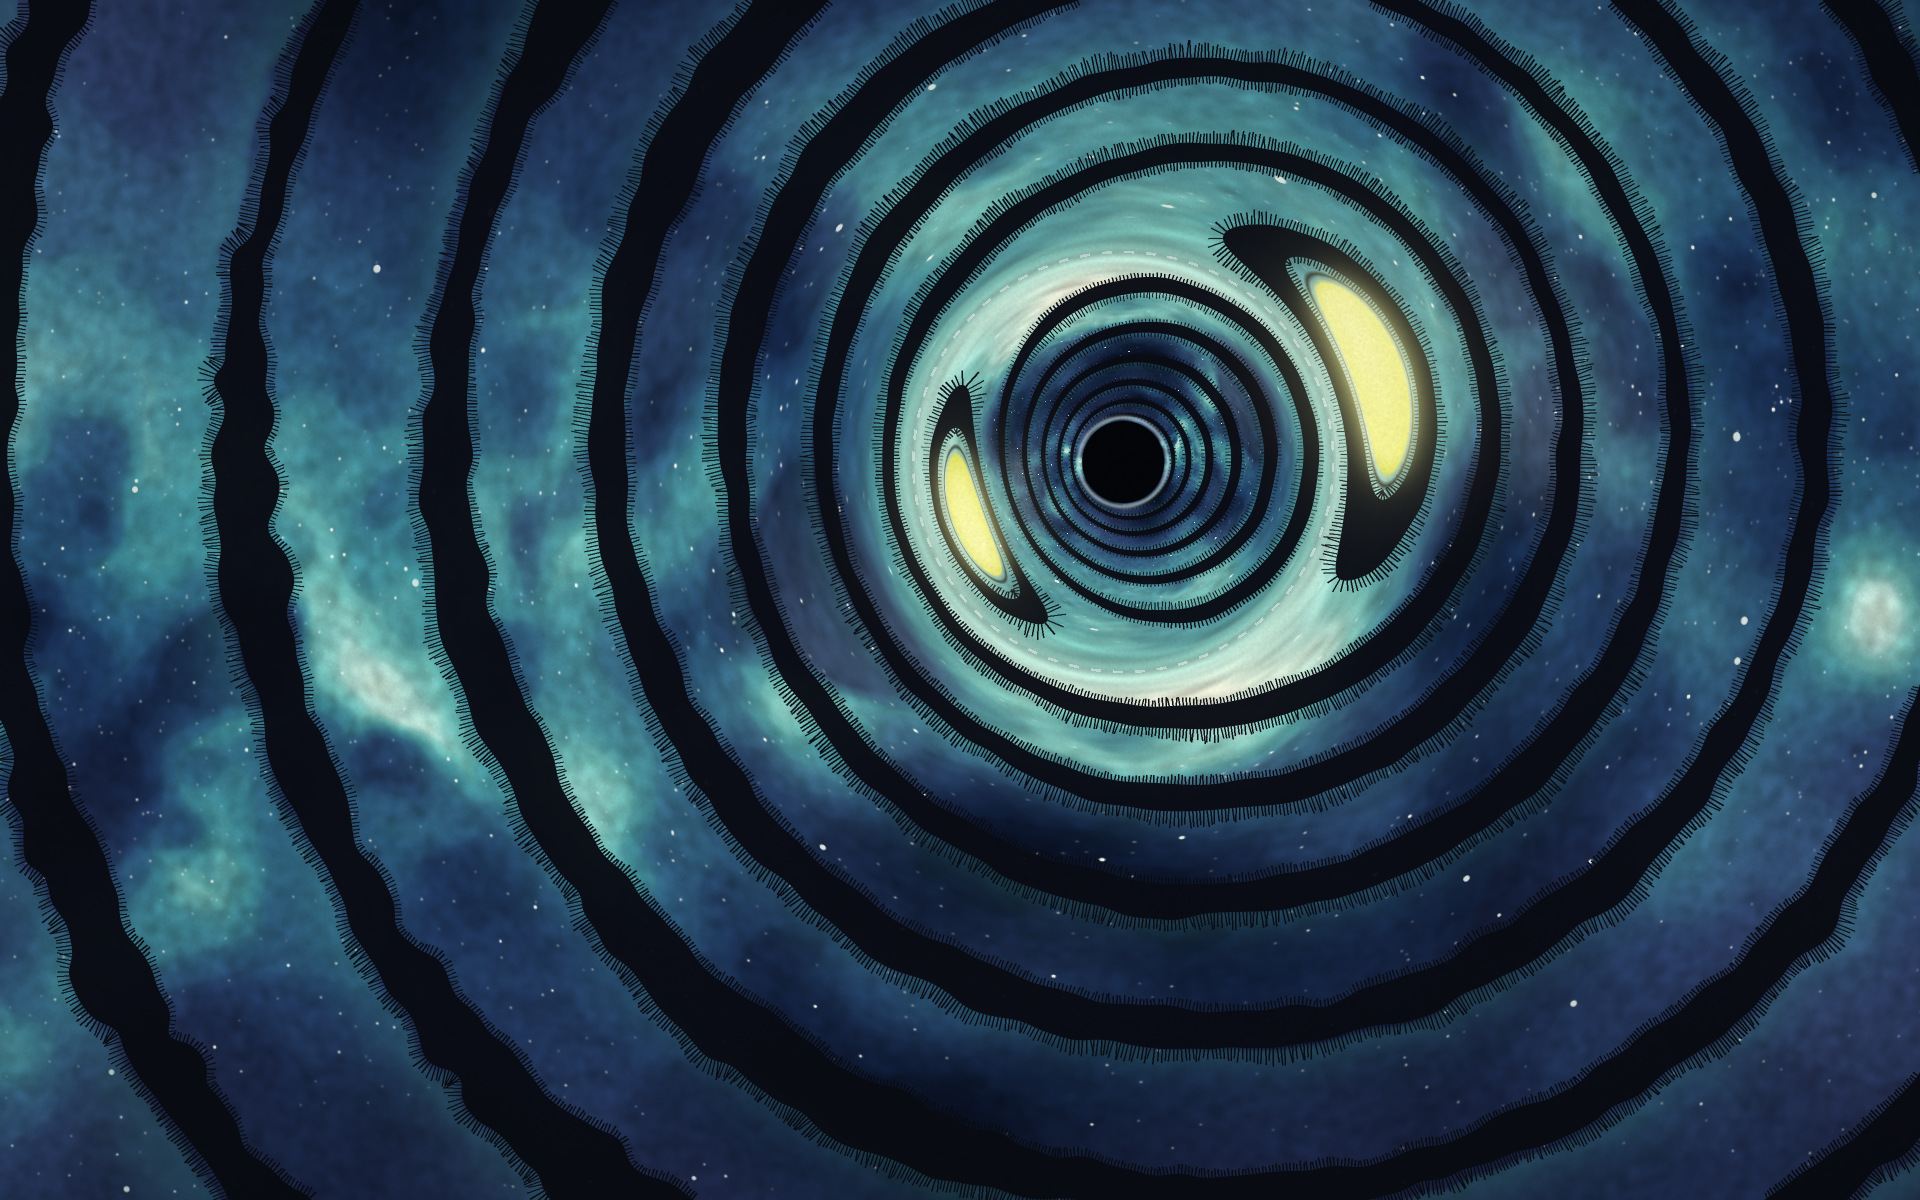
\includegraphics[width=\paperwidth,height=\paperheight]{microlensing-cartoon}}
\begin{frame}[plain]
\begin{center}
\vspace*{6.9cm}
\contourlength{2pt}
\contournumber{20}
\contour{black}{\Huge \textcolor{white}{Thank you for your attention!}}\\
\end{center}
\end{frame}
}
